% Appendix X

\chapter{Requirements Specificatie}\label{ch:requirements-specificatie}


\section{Inleiding}\label{sec:RS_inleiding}
De basis van deze analyse is de opdracht die is uitgegeven in deze opdracht zijn een aantal requirement gespecificeerd en deze zullen worden overgenomen. Daarnaast zullen er nog een aantal andere requirements zijn die door andere betrokkenen worden aangedragen. Deze zullen ook worden geanalyseeerd en desgwenest mee worden genomen in de ontwikkeling van de de nieuwe module.

\section{Huidige situatie}\label{sec:huidige-situatie}
EagleScience is al een geruime tijd bezig met het verbeteren van de buildstraat en zaken te automatiseren om zo steeds efficienter software uit te kunnen rollen. Daarnaast is het bouwen van veilige software één van de hoofdpunten waar bij EagleScience veel aandacht aan wordt besteed. Om dit te kunnen garanderen is iedere ontwikkelaar verplicht om te onderzoeken welke gevolgen het gebruik van bepaalde bibliotheken heeft op de ontwikkelde software. Dit onderzoek wordt op dit moment voor een groot deel handmatig gedaan door het uitpluizen van documentatie en registaties in een Vulnerability database op basis van de dependency declaraties in de ontwikkelde applicaties.

Dit proces is tijdrovend en de resulterende documentatie is vaak alleen op project niveau beschikbaar. Daarnaast zijn er al afgeronde applicaties die niet onder directe aandacht van het team staan, maar wel worden gehost door EagleScience. Met de tijd kunnen er kwetsbaarheben ontstaan die ongemerkt blijven bestaan. En er mogelijk pas actie wordt ondernomen als er een update van de applicatie wordt uitgevoerd door EagleScience of als er een aanval is gedaan op één van de applicaties ontwikkeld door EagleScience.

Daarnaast is de informatie die uit een SOUP analyse komt alleen makkelijk beschikbaar voor de leden van een project. Leden van andere projecten hebben dan ook niet direct beschikking tot deze informatie wat op zijn beurt kan leiden tot dubbel werk.

\section{De stakeholders}\label{sec:de-stakeholders}
Binnen EagleScience zijn er een aatal stakeholders die belang hebben bij deze nieuwe methode en module. Naast de stakeholders binnen Eaglescience is er nog een stakeholder in de vorm van de klant. Hoewel de klant niet actief is in de ontwikkeling van deze methode/module. Zij hebben er wel degelijk belang bij het resultaat en dienen ook genoemd te worden.
\subsection{Dagelijks bestuur (intern)}\label{subsec:dagelijks-bestuur-(intern)}
Het dagelijks bestuur ziet vooral voordelen in het inzicht krijgen van kwetsbaarheden op een overzichtelijke manier, zodat ze kunnen sturen in het gebruik van biblioteken of andere technologiën. Ook al zullen er kosten die niet direct terug te verdienen zijn gemoeit met de ontwikkeling van een nieuwe methode.
Echter, zien zij ook kosten gemoeid met de verandering.
Door de manier van werken dienen deze kosten terug verdient te worden door werkzaamheden binnen andere projecten.
De CTO ziet vooral tijdswinst zodat de time-to-market voor andere projecten hoger ligt en dus meer verdient kan worden.
\subsection{Projectmanagers (intern)}\label{subsec:projectmanagers-(intern)}
Project managers krijgen op dit moment een update over de staat van kwetsbaarheden tijdens stand-ups en aan het einde van een sprint tijdens de sprint demo's.
De nieuwe module biedt ze de mogelijkheid om up-to-date informatie on-demand te verkrijgen.
Op de vraag of het het waard is dat een aantal ontwikkelaars tijd kwijt zijn in testen en meedenken over de module weegt volgens hen op tegen de voordelen die de module in de toekomst kan brengen.
\subsection{Ontwikkelteam (intern)}\label{subsec:ontwikkelteam-(intern)}
Het ontwikkelteam wil graag meedenken en meewerken aan een oplossing, gezien zij de gene waren die handmatig de analyse uitvoerden.
Zij zien voor een oplossing voor een taak dat veel tijd in beslag nam en afleide van de daadwerkelijke taak.
\subsection{Klant (extern)}\label{subsec:klant-(extern)}
Als laatste de klant welke een passieve stakeholder is gezien zij niet direct betrokken zijn bij de ontwikkeling van de module maar wel verbeteringen genieten in de zin van veilige en betrouwbare software.
\subsection{Stakeholder analyse}\label{subsec:stakeholder-analyse}
\begin{figure}[H]
    \myfloatalign
    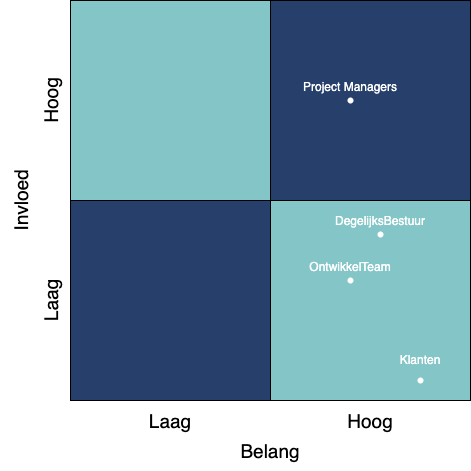
\includegraphics[width=10cm]{gfx/stakeholderanalyse}
    \caption{StakeHolders Analyse}
    \label{fig:StakeholderAnalyse}
\end{figure}
Zoals te zien is in figuur~\ref{fig:StakeholderAnalyse} zijn de projectmanager, het ontwikkelteam en de klanten het meest gebaad bij een nieuwe module voor de analyse van kwetsbaarheden.
Echter zijn de klanten niet tot bijna niet betrokken bij de ontwikkeling van de module maar hebben er indirect wel belang bij omdat de software die voor hen ontwikkeld wordt veiliger wordt door het voeren van een geautomatiseerde analyse.
Door deze analyse worden alleen de requirements meegnomen die intern zijn opgenomen.


\section{Gewenste situatie}\label{sec:gewenste-situatie}
Een situatie waar EagleScience naar toe wil is dat er periodiek of door middel van een trigger \footnote{Er kan bijvoorbeeld gedacht worden aan een commit op een branch zodat niet iedere dag een update wordt gedaan op De acceptence branche is een goed voorbeeld hiervoor} wordt onderzocht of er in de huidige dependency tree bibliotheken zitten die mogelijk kwetsbaarheden bevatten. Deze kennis dient gedeelt te worden door middel van een module in de portal die al reeds gebruikt wordt door EagleScience. Door de resultaten weer te geven in de portal ontstaat er een beter inzicht in welke bibliotheken we gebruiken en welke er potentieel kwetsbaarheden bevatten. Wat op zijn beurt weer voor veiligere applicaties kan zorgen. Ook voor de applicaties waar niet meer actief op ontwikkeld wordt. \footnote{Het is natuurlijk wel zo dat er een afhankelijk onstaat van externe bronnen die bekend moeten maken dat er een kwetsbaarheid is.}

\section{Requirements}\label{sec:requirements}
Naast het analyseren van de betrokkenheid en belang van de stakeholders is er ook gevraagd welke requirements ze terug wilden zien in de applicatie en welke prioriteit er aan gesteld werd.

Requirements kunnen worden opgedeeld in twee categoriën: "Functionele requirements" en niet-functionele requirements.

\subsection{niet functionele requirements}\label{subsec:niet-functionele-requirements}
Requirements voor de module die niet direct met de functionaliteit te maken hebben maar meer over omgevingen en dergelijke gaan.
\begin{itemize}
    \item Operationele requirements
        \begin{itemize}
            \item De methode moet zonder veel aanpassingen passen in de huidige werkstroom voor het ontwikkelen van software.
        \end{itemize}
    \item Omgeving requirements
        \begin{itemize}
            \item De module dient te worden ontwikkeld in Angular en Play(Scala), overeenkomstig met bestaande portal.
            \item De module dient gescheiden componenten te bevatten: Frontend(Angular), Backend(Play, Scala), API.
            \item De module dient in het Azure cluster te kunnen draaien binnen het huidige portal project.
        \end{itemize}
    \item Performance requirements
        \begin{itemize}
            \item De module moet op een zo efficient mogelijke manier een raport genereren.
            \item De module mag geen invloed hebben op de performance van de buildstraat.
        \end{itemize}
    \item security requirements
        \begin{itemize}
            \item Er dienen geen persoonsgegevens opgeslagen te worden die niet nodig zijn voor het functioneren van de module.
            \item Source code dient minimaal 70\% test coverage te hebben.
        \end{itemize}
\end{itemize}

\subsection{functionele requirements}\label{subsec:functionele-requirements}
\begin{itemize}
    \item De module dient eenvoudig gebruikt te kunnen worden in de huidige CI/CD pipeline voor bestaande en nieuwe projecten.
    \item De module dient ondersteuning te bieden voor meerdere omgevingen (OTAP)
    \item De module dient met een instelbaar interval een analyse uit te voeren op bestaande projecten.
    \item De module moet op project en omgevings niveau te rapporteren over bekende kwetsbaarheden.
    \item De module dient kwetsbaarheden op minimaal drie niveau's in te schalen(Kritish, gemiddeld en laag)
    \item De module dient ondersteuning te bieden voor het instellen van quality gates over meldingen die het vind op ieder niveau, per project, per omgeving.
\end{itemize}


\section{User stories}\label{sec:user-stories}
Naast de requirements uit de vorige sectie zijn er de volgende userstories opgetekend welke aangeven dat als deze geimplementeerd worden de module bruikbaar is voor de verschillende belanghebbenden. De userstories zijn onderverdeeld middels het MoSCoW principe.

\textbf{Must Have}
\begin{itemize}
    \item Als \textit{gebruiker} wil ik dat de SOUP-module in de portal te vinden is zodat alle tools die gebruikt worden binnen Eaglescience op een enkele plek te vinden zijn.
    \item Als \textit{gebruiker} wil ik een overzicht per project kunnen zien met daarin de gebruikte bibliotheken zodat ik inzage heb ik wat er gebruikt wordt voor ontwikkeling.
    \item Als \textit{gebruiker} wil ik een overzicht per project zien welke kwetsbaarheden er zich in bibliotheken bevinden, zodat ik actie kan ondernemen om de software nog veiliger te maken.
    \item Als \textit{gebruiker} wil ik in kunnen loggen met mijn LDAP account zodat ik niet nog een keer een username/wachtwoord combinatie hoe te leren.
    \item Als \textit{gebruiker} wil ik een project kunnen toevoegen zodat ik ook van dat project de kwetsbaarheden in kan zien en deze software ook veilger wordt.
    \item Als \textit{Module} wil ik een update krijgen van de laatste build met specifiek de laatste kwetsbaarheden, zodat ik deze kan weergeven in de portal.
    \item Als \textit{module} wil ik
    \item Als \textit{gebruiker} wil ik dat periodiek automatisch een check analyse wordt uitgevoerd zodat ik er zelf niet naar om hoef te kijken.
    \item Als \textit{gebruiker} wil ik zelf een analyse kunnen starten voor een project zodat ik een up-to-date versie heb van de resultaten.
    \item Als \textit{Project manager} wil ik projecten kunnen toevoegen aan de module, zodat ook deze mee genomen worden in de automatische analyse.
    \item Als \textit{Project manager} wil ik ontwikkelaars kunnen toevoegen aan een project zodat deze ook inzicht krijgen in de huidige stand van zaken.
    \item Als \textit{Project manager} wil ik een notificatie( via mail/rocketchat) ontvangen als er een kritieke kwetsbaarheid gevonden is.
\end{itemize}

\textbf{Should Have}
\begin{itemize}
    \item Moeten nog voorkomen uit de prioriteit analyse
\end{itemize}

\textbf{Could Have}
\begin{itemize}
    \item
\end{itemize}

\textbf{Won't Have}
\begin{itemize}
    \item Moeten nog voorkomen uit de prioriteit analyse
\end{itemize}
De Won't haves staan hierbij genoemd als leidraad voor eventueel updates in de toekomst.
Als blijkt dat er tussen de won'ts toch low hanging fruit blijkt te hangen kunnen deze meegenomen worden in de sprints.
De requirements worden als epics in een JIRA-omgeving gezet om vervolgens een planning te kunnen maken.


